\begin{song}{title=\predtitle\centering Franky Dlouhán \\\large Brontosauři  \vspace*{-0.3cm}}  %% sem se napíše jméno songu a autor
\begin{centerjustified}
\nejvetsi

\sloka 
	^{C}Kolik je smutného,
	
	když ^{F{\color{white}\_\_}}mraky černé ^{C}jdou

	lidem nad ^*{G}hl avou ^{F{\color{white}\_\_\_}}smutnou dálavo^{C}u.
	
	Já slyšel příběh, který velkou pravdu měl,
	
	za čas odletěl, každý zapomněl.

\refren
	^{C}Měl kapsu ^*{G}pr ázdnou Franky Dlouhán,

	po státech ^*{F}to ulal se jen ^{C}sám, a že

	byl ^*{F}ve selej, tak ^*{C}ka ždej měl ho ^{G7}rád.

	Tam ruce k ^{F\,\,\,}dílu mlčky přiloží a ^{C\,\,\,}zase

	jede ^{Ami}dál. A ^*{F}ka ždej kdo s ním

	^*{G}ch vilku byl, tak ^*{F}dl ouho ^{G7}se pak ^{C\,\,\,}smál.
	
\sloka	
	Tam, kde byl pláč, tam Franky hezkou píseň měl,
	
	slzy neměl rád, chtěl se jenom smát.
	
	A když pak večer ranče tiše usínaj,
	
	Frankův zpěv jde dál nocí s písní dál.\elipsa\dots
	
\sloka
	Tak Frankyho vám jednou našli, přestal žít,
	
	jeho srdce spí, tiše smutně spí.
	
	Bůh ví jak, za co tenhle smíšek konec měl,
	
	farář píseň pěl, umíraček zněl.\elipsa\dots

\end{centerjustified}
\setcounter{Slokočet}{0}
\end{song}


\begin{figure}[h]
\centering
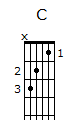
\includegraphics[width=3cm]{../Akordy/c.png}
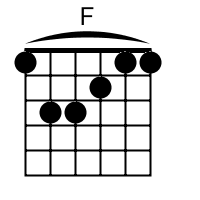
\includegraphics[width=3cm]{../Akordy/f.png}
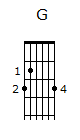
\includegraphics[width=3cm]{../Akordy/g.png}
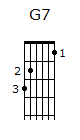
\includegraphics[width=3cm]{../Akordy/g7.png}
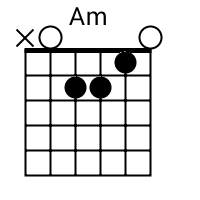
\includegraphics[width=3cm]{../Akordy/am.png}
\end{figure}
